
\documentclass[10pt,a4paper]{article}

\usepackage[a4paper,margin=0.68in,headheight=13pt]{geometry}
\usepackage[T1]{fontenc}
\usepackage[utf8]{inputenc}
\usepackage{lmodern}
\usepackage{microtype}
\usepackage{setspace}
\usepackage{graphicx}
\usepackage{xcolor}
\usepackage{booktabs}
\usepackage{longtable}
\usepackage{tabularx}
\usepackage{array}
\usepackage{enumitem}
\usepackage{float}
\usepackage{caption}
\usepackage{subcaption}
\usepackage{listings}
\usepackage{fancyhdr}
\usepackage{titlesec}
\usepackage{hyperref}
\usepackage{url}
\usepackage{amsmath}
\usepackage{amssymb}
\usepackage{pdflscape}
\usepackage{multirow}
\usepackage{makecell}
\usepackage{lastpage}

\definecolor{codebg}{RGB}{246,246,246}
\definecolor{codegray}{RGB}{75,75,75}
\definecolor{linkblue}{RGB}{25,70,130}

\hypersetup{
  colorlinks=true,
  linkcolor=linkblue,
  citecolor=linkblue,
  urlcolor=linkblue,
  pdftitle={Design Pattern Analysis and Evolution in a Ruby on Rails Hotel Booking Application},
  pdfauthor={Team A7}
}

\lstset{
  backgroundcolor=\color{codebg},
  basicstyle=\ttfamily\small,
  breaklines=true,
  columns=fullflexible,
  keepspaces=true,
  frame=single,
  rulecolor=\color{gray!35},
  numbers=left,
  numberstyle=\tiny\color{codegray},
  xleftmargin=2em,
  framexleftmargin=1.5em
}

\pagestyle{fancy}
\fancyhf{}
\lhead{23CSE455 -- Design Pattern Case Study}
\rhead{Team A7}
\cfoot{\thepage\ of \pageref{LastPage}}

\titleformat{\section}{\large\bfseries}{\thesection}{0.7em}{}
\titleformat{\subsection}{\normalsize\bfseries}{\thesubsection}{0.6em}{}
\setstretch{1.0}\sloppy

\newcommand{\code}[1]{\texttt{\small #1}}
\newcommand{\verified}{\textbf{Verified}}
\newcommand{\notverified}{\textbf{Not verified from the available source/evidence}}
\newcommand{\repo}{\url{https://github.com/andrewdsilva/rails-room-booking}}
\newcommand{\baseline}{\code{5e15551ee646871b4bed32c982fa17da319d3ee3}}

\begin{document}

% ---------------- TITLE PAGE ----------------
\hypersetup{pageanchor=false}
\begin{titlepage}
\centering
\vspace*{1.0cm}
{\Large\bfseries 23CSE455 -- Design Pattern Case Study\par}
\vspace{1.2cm}
{\LARGE\bfseries Design Pattern Analysis and Evolution in a Ruby on Rails Hotel Booking Application\par}
\vspace{1.4cm}
{\large Final Academic Report\par}
\vspace{1.2cm}

\begin{tabular}{ll}
\textbf{Team} & A7\\
\textbf{Programme / Batch} & B.Tech Artificial Intelligence \& Data Science (AI \& DS)\\
\textbf{Application} & \code{rails-room-booking}\\
\textbf{Source language} & Ruby / Ruby on Rails\\
\textbf{Part 3 languages} & Java, Python, JavaScript, C++\\
\textbf{Baseline commit} & \code{5e15551ee646871b4bed32c982fa17da319d3ee3}\\
\textbf{Document revision} & 2026-10-11 (current repair; not an original submission date)\\
\textbf{Submission date} & Not verified from retained inputs
\end{tabular}

\vfill
{\large\bfseries Team Members\par}
\vspace{0.3cm}
\begin{tabular}{lll}
\toprule
Roll Number & Name & Batch\\
\midrule
AM.AI.U4AID23016 & Kavya Penikalapati & AI \& DS\\
AM.AI.U4AID23037 & E. Abhijith Krishna & AI \& DS\\
AM.AI.U4AID23040 & Guduru Akshaya Giri & AI \& DS\\
AM.AI.U4AID23046 & Kurt Sony Rebello & AI \& DS\\
\bottomrule
\end{tabular}

\vfill
\textit{Prepared as an evidence-based software engineering case study.}
\end{titlepage}

\pagenumbering{roman}
\hypersetup{pageanchor=true}
\cfoot{\thepage}
\tableofcontents
\clearpage
\listoffigures
\clearpage
\listoftables
\clearpage
\pagenumbering{arabic}
\cfoot{\thepage\ of \pageref{LastPage}}

% ---------------- EXECUTIVE SUMMARY ----------------
\section{Executive Summary}

This case study investigates the architecture and design-pattern structure of \code{rails-room-booking}, an open-source Ruby on Rails hotel/room booking application. The study uses an immutable source baseline rather than treating the current repository state as an informal reference: the original application is identified by repository \repo{} and commit \baseline. The investigation covers the application's domain model, controllers, Rails concerns, authentication and authorization mechanisms, payment integration, notification integration, and booking lifecycle.

The central methodological decision was to distinguish framework mechanisms and ordinary object-oriented reuse from application-level Gang of Four (GoF) design patterns. A pattern was confirmed only when its participant roles, interactions, source locations, and behavioral purpose could be established from the source. This prevents a common failure mode in design-pattern assignments in which every callback is called Observer, every policy class is called Strategy, or every wrapper is called Decorator or Adapter.

Under that evidence standard, the baseline contains \textbf{one clearly confirmed application-level GoF collaboration: Template Method}. The collaboration is the shared CRUD workflow implemented by \code{CrudConcern} and specialized by \code{BookingsController}, \code{RoomsController}, and \code{SettingsController}. \code{CrudConcern} provides the common algorithm through actions such as \code{index}, \code{show}, \code{new}, \code{create}, \code{edit}, \code{update}, and \code{destroy}; concrete controllers provide hook methods such as \code{base\_class}, \code{object\_class}, \code{strong\_params}, \code{model\_params}, \code{use\_slug?}, \code{set\_object}, and \code{redirect\_to\_show}. The use of explicit \code{NotImplementedError} extension points further demonstrates that the common workflow is intentionally parameterized by resource-specific operations.

The second part evolves the design for four realistic requirements: a breakfast package, an airport transfer, room upgrades, and configurable cancellation policies. The first two are modeled as optional additional services rather than permanent room attributes. Room upgrade is isolated as a reservation-domain operation. Cancellation is the strongest case for a new GoF pattern: a \code{CancellationService} delegates variable cancellation and refund behavior to a \code{CancellationPolicy}, with concrete policies for flexible, partial-refund, and no-refund rules. This establishes a genuine \textbf{Strategy} collaboration because the context delegates the same conceptual operation to interchangeable algorithms. The complete evolved Rails application passed 36 RSpec examples with zero failures, including 30 feature examples and an eager-loading check, after rebuilding the dedicated PostgreSQL test database from all 12 migrations.

The third part reproduces the two confirmed pattern ideas independently in Java, Python, JavaScript, and C++. The implementations do not attempt to port the entire Rails application. Instead, they preserve the pattern intent and representative behavior. Eight snippets were executed: four Template Method implementations and four Strategy implementations. Each passed its specified behavioral check. Process-level timing used one warmup followed by five measured runs, with the median reported. The measured medians show substantial runtime differences between languages, but these observations are environment-dependent and are not interpreted as universal language-speed claims.

LLM assistance was used as an analytical aid for source exploration, candidate pattern discovery, evolution reasoning, cross-language implementation, and final audit. The human-verification rule was retained throughout: an LLM hypothesis was not treated as evidence until checked against source code or executable artifacts. Historical Prompt 02 and Prompt 03 wording could not be recovered verbatim from the retained records, so this report explicitly records that limitation rather than fabricating a transcript.

The result is intentionally conservative. The project demonstrates that a smaller pattern inventory can be more academically defensible than a larger inventory produced by pattern-by-name classification. It also demonstrates that new requirements do not necessarily justify forcing every new class into a GoF pattern: additional services and room upgrade are primarily domain-modeling/refactoring decisions, while cancellation-policy variation has the structural and behavioral characteristics required for Strategy.

% ---------------- INTRODUCTION ----------------
\section{Introduction}

\subsection{Design patterns and evidence-based identification}

Software design patterns are reusable descriptions of design structures that solve recurring problems in a context. Their value is not in assigning familiar names to arbitrary classes; the value lies in recognizing a recurring collaboration and understanding the trade-offs that motivate it. In an academic case study, this distinction is particularly important because a framework such as Ruby on Rails already provides conventions, lifecycle callbacks, inheritance, concerns, routing, persistence and dependency mechanisms. These mechanisms can resemble design-pattern vocabulary without necessarily constituting an application-level GoF pattern.

The present study therefore treats pattern identification as an evidence problem. A candidate must have recognizable participant roles, interactions between those participants, a behavioral or structural purpose corresponding to the pattern intent, and source evidence that demonstrates the collaboration. A class name such as \code{Policy} is not enough to prove Strategy; a callback is not automatically Observer; and a concern is not automatically Decorator.

\subsection{Case-study purpose}

The purpose of the case study is to investigate an existing hotel booking application, identify the patterns that can actually be defended from source evidence, evolve the design under new requirements, and compare representative implementations across four programming languages.

The study objectives are:

\begin{enumerate}[leftmargin=*]
\item Analyze the architecture of an existing hotel booking application.
\item Identify design patterns actually present in the source.
\item Distinguish genuine patterns from superficial pattern candidates.
\item Evolve the application in response to new requirements.
\item Determine whether new design patterns become justified after evolution.
\item Implement representative confirmed patterns in Java, Python, JavaScript and C++.
\item Compare the implementations using structural, behavioral and process-level performance evidence.
\end{enumerate}

These are study objectives, not claims that the expected outcomes were known before the investigation.

\subsection{Three-part assignment structure}

The investigation is divided into three parts. Part 1 establishes a reproducible baseline and performs pattern discovery. Part 2 introduces new domain requirements and evaluates the resulting design pressure, including a Strategy-based cancellation-policy design. Part 3 isolates the confirmed pattern collaborations into small executable examples so that the same design intent can be compared across four languages.

% ---------------- APPLICATION ----------------
\section{Application and Architecture}

\subsection{Application background}

The studied application is \code{rails-room-booking}, an existing Ruby on Rails hotel/room booking application. The baseline source is the public repository \repo{} at commit \baseline. The source language is Ruby and the application uses Rails MVC and Active Record as its main application architecture.

The baseline domain entities established directly from the inspected source are:

\begin{itemize}[leftmargin=*]
\item \textbf{User}: authenticated application user and owner of rooms/bookings/settings.
\item \textbf{Room}: bookable accommodation with descriptive attributes, capacity, pricing and amenity flags.
\item \textbf{Booking}: reservation connecting a user and room, with dates, guests, price totals and cancellation state.
\item \textbf{Setting}: user-associated configuration, including VAT used by booking-price calculation.
\end{itemize}

The baseline source does \textbf{not} establish separate application-owned models for Hotel, Customer, Cancellation, or AdditionalService. This distinction matters because the case study must not retroactively attribute domain objects to the application merely because those concepts appear in the assignment statement.

\subsection{Baseline source and reproducibility}

The immutable baseline is:

\begin{center}
\begin{tabular}{ll}
\toprule
Repository & \repo\\
Baseline commit & \baseline\\
Application language & Ruby\\
Framework & Ruby on Rails\\
Ruby version in baseline Gemfile & 2.7.5\\
Rails dependency in baseline Gemfile & \code{\textasciitilde7.0.4}\\
Database at baseline commit & PostgreSQL\\
\bottomrule
\end{tabular}
\end{center}

The database conclusion is supported by the baseline commit itself: that commit changes the application from SQLite to PostgreSQL, adds the \code{pg} dependency, changes \code{code/config/database.yml}, and adds a PostgreSQL service to Docker Compose. The source therefore supports describing PostgreSQL as the baseline database configuration.

The complete baseline source is retained under \code{code/}; the complete evolved Rails application is retained under \code{Part2/code/}. The inspected application areas include the main domain models, controllers and controller concerns, routing, schema, selected model specifications and the relevant dependency configuration. External-library internals were not treated as observable application source.

\subsection{Architecture overview}

The baseline follows the conventional Rails flow:

\begin{figure}[H]
\centering
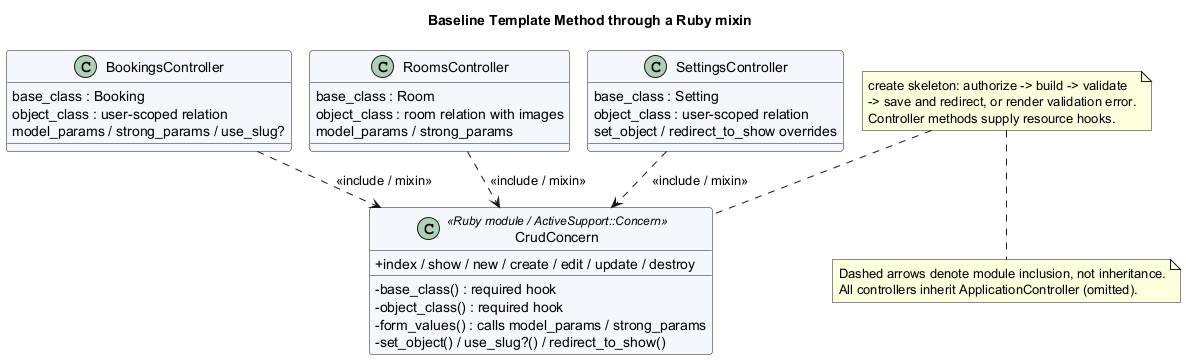
\includegraphics[width=0.84\linewidth]{Part1/pattern_architecture.png}
\caption{Baseline Template Method collaboration implemented by Ruby module inclusion. Dashed dependencies denote \code{include CrudConcern}, not class inheritance; controller hooks specialize the shared CRUD skeleton.}
\label{fig:baseline-architecture}
\end{figure}

At a high level, a browser request reaches Rails routes and a controller. Controllers use Active Record models and model concerns to access and manipulate persistent state. PostgreSQL stores the application data. Pundit is used for authorization, Devise for authentication, Payify/Stripe integration for payments, Active Storage for attachments, and Integromat/Make integration for booking webhooks. Stimulus and Turbo participate in the front-end interaction model.

The architecture is therefore better described as a Rails MVC/Active Record application with reusable concerns and integrations than as a collection of GoF patterns. This framing is important because Rails itself supplies substantial structure.


\begin{figure}[H]
\centering
\fbox{\begin{minipage}{0.88\linewidth}
\centering
\textbf{Baseline Application Architecture}\\[0.35cm]
\begin{tabular}{c}
\framebox{\strut Browser}\\
$\downarrow$\\
\framebox{\strut Rails Routes}\\
$\downarrow$\\
\framebox{\strut Controllers}\\
$\downarrow$\\
\begin{tabular}{ccc}
\framebox{\strut Active Record Models} &
\hspace{0.25cm}\framebox{\strut Controller Concerns} &
\hspace{0.25cm}\framebox{\strut Model Concerns}
\end{tabular}\\
$\downarrow$\\
\framebox{\strut PostgreSQL}
\end{tabular}

\vspace{0.35cm}
\begin{tabularx}{0.88\linewidth}{XXX}
\centering
Devise authentication & Pundit authorization & Payify/Stripe payment\\
Active Storage & Stimulus/Turbo & Integromat/Make webhook
\end{tabularx}
\end{minipage}}
\caption{Baseline application architecture reconstructed from the inspected Rails source. External integrations are shown as boundaries; their internal implementations are not assumed.}
\label{fig:baseline-architecture-overview}
\end{figure}

\subsection{Major framework and integration mechanisms}

\begin{table}[H]
\centering
\caption{Baseline framework mechanisms and their role}
\label{tab:framework}
\begin{tabularx}{\linewidth}{lX}
\toprule
Mechanism & Evidence-backed role\\
\midrule
Rails MVC & Routes requests to controllers and renders/redirects responses.\\
Active Record & Maps application models to persistent relational data and provides associations/querying.\\
Devise & Authentication/user-account mechanism referenced by the application.\\
Pundit & Authorization mechanism used by controllers through \code{authorize}.\\
Payify / Stripe & Payment integration visible through the Booking payment concern and payment controller/engine.\\
Active Storage & Room image attachments.\\
Integromat / Make & Booking webhook integration visible in \code{Booking\#notify\_booking}.\\
Stimulus / Turbo & Front-end interaction mechanisms included by the Rails application.\\
Controller concerns & Reusable controller behavior, including the shared CRUD workflow.\\
Model concerns & Reusable model behavior, including pricing/ownership/settings-related logic.\\
\bottomrule
\end{tabularx}
\end{table}

The table deliberately labels these as framework or integration mechanisms. Their presence does not automatically imply a corresponding GoF pattern.

\subsection{Architecture collaborations}

\subsubsection{User and Booking}

The source establishes \code{Booking belongs\_to :user} and \code{User has\_many :bookings}. The booking controller also scopes booking queries by \code{current\_user.id}. This provides both persistence-level association and controller-level ownership scoping.

\subsubsection{User and Room}

The source establishes \code{Room belongs\_to :user} and \code{User has\_many :rooms}. This relationship supports room ownership and the room-management scope.

\subsubsection{Room and Booking}

The source establishes \code{Room has\_many :bookings} and \code{Booking belongs\_to :room}. Availability is checked in \code{Booking\#dates\_are\_available}, where conflicting bookings are queried using the candidate booking's dates. \code{Room\#booked\_dates} separately exposes future booked date ranges in a display-oriented representation.

\subsubsection{Booking and Setting}

Pricing behavior is extracted into \code{HasPriceConcern}. Its \code{vat} method accesses \code{room.user.setting.vat}, making the setting part of the booking-price calculation.

\subsubsection{Booking and Payify}

\code{Booking} includes \code{Payify::HasPaymentConcern}. The source also defines \code{payment\_pending?}, \code{paid?}, \code{amount\_to\_pay} and the \code{stripe\_init\_intent} controller hook. The internal implementation of Payify/Stripe is not treated as part of the observable application pattern evidence.

\subsubsection{Booking and Integromat}

The Booking model contains \code{after\_create :notify\_booking}. The \code{notify\_booking} method checks for the configured booking webhook and invokes \code{Integromat::Webhook.new(:booking).trigger(...)}. This establishes an observable integration, but it does not by itself prove an Observer pattern.

\subsubsection{Controllers and CrudConcern}

The controllers include \code{CrudConcern}, a Ruby module using \code{ActiveSupport::Concern}. The module is mixed into each controller; it is not a superclass, and no \code{CrudTemplate} interface exists in the source. Its public CRUD actions preserve the algorithmic skeleton while private helper methods and controller hook overrides supply resource-specific behavior. All three controllers inherit \code{ApplicationController} independently of module inclusion. This collaboration is the strongest baseline GoF pattern evidence.

\subsubsection{Controllers and Pundit}

The CRUD workflow and the booking cancellation action call \code{authorize}. This demonstrates an authorization collaboration, but the available source does not establish the participant structure required to call the Pundit policy hierarchy a Strategy instance in the baseline.

\subsection{Important baseline flows}

\subsubsection{Booking creation}

The observable booking-creation path is:

\begin{center}
\code{Request -> Route -> BookingsController -> CrudConcern\#create -> authorize -> Booking.new -> validation -> save -> callbacks -> redirect}
\end{center}

The controller delegates the common create algorithm to the concern. Booking-specific behavior enters through \code{object\_class}, \code{strong\_params}, \code{model\_params}, and the model's own validations/callbacks.

\subsubsection{Availability}

The availability validation is performed by \code{Booking\#dates\_are\_available}. It queries the room's existing bookings and rejects a new booking when date intervals overlap.

\begin{lstlisting}[language=Ruby,caption={Verified baseline excerpt: booking availability validation}]
def dates_are_available
  conflicting_bookings = room.bookings.where.not(id: id).
    where("(? < end_date) AND (? > start_date)", start_date, end_date)

  errors.add(:base, I18n.t(
    "activerecord.errors.models.booking.unavailable_dates"
  )) if conflicting_bookings.exists?
end
\end{lstlisting}

\subsubsection{Cancellation}

The baseline cancellation flow is:

\begin{center}
\code{POST /bookings/:id/cancel -> BookingsController\#cancel -> authorize -> Booking\#cancel! -> canceled\_at -> redirect}
\end{center}

The baseline implementation simply records cancellation time through \code{update\_attribute :canceled\_at, Time.now}. There is no application-owned cancellation-policy hierarchy in the baseline source.

\subsubsection{Payment}

Payment behavior is partially delegated to the Payify concern. The Booking model includes the concern, and the controller invokes a Stripe initialization operation when the payment is pending. Because Payify/Stripe internals are external, the report does not claim an application-level Adapter, Facade or Strategy pattern inside those dependencies.

\subsubsection{Booking notification}

\begin{center}
\code{Booking creation -> after\_create -> notify\_booking -> Integromat webhook}
\end{center}

This is an observable callback-to-integration path. It is intentionally classified as a framework/application callback mechanism rather than Observer because the required observer/subject collaboration is not established by the inspected source.

% ---------------- PART 1 ----------------
\section{Part 1 -- Pattern Discovery}

\subsection{Discovery method}

The pattern-discovery method follows a source-first procedure:

\begin{enumerate}[leftmargin=*]
\item Establish an immutable source baseline.
\item Identify candidate collaborations from controllers, models, concerns and service boundaries.
\item Trace calls and overrides between candidate participants.
\item Map the observed roles to the recognized pattern intent.
\item Record source locations and behavioral purpose.
\item Reject candidates when required participant/delegation evidence is absent.
\item Verify the final inventory independently against the source.
\end{enumerate}

The central methodological rule is:

\begin{quote}
A pattern is not confirmed from class names, annotations, inheritance, Rails conventions, or an LLM assertion alone. Confirmation requires participant roles, actual source locations, actual interactions, delegation/calls, behavioral purpose, and correspondence with the recognized pattern.
\end{quote}

This produces a smaller but more defensible inventory.

\subsection{Baseline result}

The baseline investigation confirmed exactly \textbf{one GoF pattern type and one pattern instance}:

\begin{table}[H]
\centering
\caption{Baseline pattern inventory}
\label{tab:baseline-pattern}
\begin{tabularx}{\linewidth}{lX}
\toprule
Field & Verified result\\
\midrule
Pattern & Template Method\\
Category & Behavioral\\
Instance & Shared CRUD Controller Workflow\\
Template holder & \code{CrudConcern}\\
Concrete participants & \code{BookingsController}, \code{RoomsController}, \code{SettingsController}\\
Count of confirmed pattern types & 1\\
Count of confirmed pattern instances & 1\\
\bottomrule
\end{tabularx}
\end{table}

\subsection{Template Method -- detailed analysis}

\subsubsection{Participant roles}

The template holder is \code{CrudConcern}. The concrete participants are \code{BookingsController}, \code{RoomsController}, and \code{SettingsController}.

The concern provides the common CRUD algorithm:

\begin{itemize}[leftmargin=*]
\item \code{index}
\item \code{show}
\item \code{new}
\item \code{create}
\item \code{edit}
\item \code{update}
\item \code{destroy}
\end{itemize}

The extension points include:

\begin{itemize}[leftmargin=*]
\item \code{base\_class}
\item \code{object\_class}
\item \code{strong\_params}
\item \code{model\_params}
\item \code{use\_slug?}
\item \code{set\_object}
\item \code{redirect\_to\_show}
\end{itemize}

The baseline source locations are:

\begin{table}[H]
\centering
\caption{Template Method source evidence}
\label{tab:tm-evidence}
\begin{tabularx}{\linewidth}{lX}
\toprule
Participant & Verified source range\\
\midrule
Template holder: \code{CrudConcern} & \code{code/app/controllers/concerns/crud\_concern.rb:1--149}\\
Concrete: \code{BookingsController} & \code{code/app/controllers/bookings\_controller.rb:1--47}\\
Concrete: \code{RoomsController} & \code{code/app/controllers/rooms\_controller.rb:1--41}\\
Concrete: \code{SettingsController} & \code{code/app/controllers/settings\_controller.rb:1--39}\\
\bottomrule
\end{tabularx}
\end{table}

\subsubsection{Why this is Template Method}

The collaboration has the essential shape of Template Method even though Ruby/Rails expresses it through a module concern rather than a Java-style abstract class.

First, the reusable algorithm is centralized. For example, \code{create} performs authorization, constructs an object, validates it, saves it, and redirects on success; otherwise it renders the form with an error status. The algorithm is not copied separately into each resource controller.

Second, the algorithm invokes resource-specific hooks. \code{object\_class}, \code{strong\_params} and \code{model\_params} determine which resource and parameters participate in the shared lifecycle.

Third, the concrete controllers implement those hooks differently. Their \code{base\_class} methods return \code{Booking}, \code{Room}, and \code{Setting}, respectively; their \code{object\_class} methods return the corresponding scoped Active Record relations. \code{SettingsController} additionally overrides \code{set\_object} and \code{redirect\_to\_show} because its resource semantics differ.

Fourth, the concern contains explicit required extension points. \code{base\_class} and \code{object\_class} raise \code{NotImplementedError} in the shared module. This is stronger evidence than mere code reuse: it establishes a reusable algorithm with designated operations that concrete participants must supply.

\begin{lstlisting}[language=Ruby,caption={Verified baseline Template Method hook structure}]
def base_class
  raise NotImplementedError
end

def object_class
  raise NotImplementedError
end

def use_slug?
  true
end
\end{lstlisting}

The pattern therefore represents a deliberate collaboration: a fixed workflow is preserved while resource-specific details vary.

\subsection{Concrete controller specialization}

\code{BookingsController} specializes the template with Booking-specific querying, permitted parameters and non-slug lookup. It also adds a booking-specific cancellation action and Stripe payment initialization.

\code{RoomsController} specializes the template with Room-specific querying, image attachment handling and room parameters. It also adds booking-form initialization for a room.

\code{SettingsController} specializes the template with Setting-specific lookup and redirects. Its \code{set\_object} implementation obtains the current user's setting and its \code{redirect\_to\_show} redirects to the settings path rather than a polymorphic resource show page.

This variation is exactly why the shared algorithm is useful: the common CRUD sequence is stable while resource-specific behavior is localized.

\subsection{Why this is more than ordinary reuse}

A generic helper function could reduce duplication without being Template Method. The distinguishing evidence here is that the shared concern owns the workflow and explicitly defines a family of operations that concrete controllers supply or override. The concrete classes are not simply calling a utility; they participate in a common algorithmic skeleton.

This distinction is important in the academic classification. The report therefore identifies Template Method rather than simply saying that \code{CrudConcern} is ``reusable code.''

\subsection{Rejected and uncertain candidates}

\begin{longtable}{p{0.22\linewidth}p{0.31\linewidth}p{0.38\linewidth}}
\caption{Rejected or uncertain baseline candidates}
\label{tab:rejected}\\
\toprule
Candidate & Initial suggestion & Reason not confirmed\\
\midrule
Strategy via Pundit & Policies and \code{authorize} suggest policy-based behavior. & The inspected application does not establish a Strategy context delegating a common operation to interchangeable policy algorithms.\\
Strategy via CrudConcern hooks & Hook methods vary by controller. & The variation belongs to the Template Method mechanism; the shared CRUD algorithm is not selecting interchangeable algorithms at runtime.\\
Policy inheritance & Pundit policies form an authorization structure. & Inheritance alone is insufficient; the required interchangeable algorithm collaboration was not established.\\
Observer & \code{after\_create} and \code{after\_save} callbacks trigger side effects. & Rails callbacks are lifecycle hooks; the source does not establish a subject maintaining and notifying observer objects.\\
Adapter & Payify/Stripe integration looks like an external interface boundary. & Payify internals are external and not observable as an application-owned adapter collaboration.\\
Facade & Payment functionality is accessed through a higher-level concern. & No application-owned facade abstraction was established from the inspected source.\\
Decorator & Rails concerns wrap/add model behavior. & The concern mechanism is not demonstrated as runtime wrapping of component objects.\\
Composite & Active Record associations form object relationships. & Associations do not establish the recursive uniform part-whole structure required by Composite.\\
Factory Method / Abstract Factory & Rails constructors and persistence helpers create objects. & No dedicated application-owned factory collaboration with varying creation products was established.\\
Command & Controller actions represent operations. & A controller action is not automatically a Command object with encapsulated request/operation state.\\
State & Booking has states such as paid/pending/canceled. & No state-object hierarchy or state-dependent polymorphic delegation is present in the baseline.\\
Memento & Booking persists state. & Persistence alone is not an object-state snapshot/restore collaboration.\\
Chain of Responsibility & Request processing passes through Rails layers. & Framework request flow does not establish a chain of interchangeable handlers in the application code.\\
Prototype & Active Record objects can be duplicated. & No prototype-based object creation mechanism is established.\\
Singleton & Rails configuration objects are globally accessible. & Framework singleton-like services are not evidence of an application-owned Singleton implementation.\\
\bottomrule
\end{longtable}

The rejected-candidate analysis is not a claim that these patterns are impossible in Rails. It is a claim about what can be defended from this particular baseline source.

% ---------------- PART 2 ----------------
\section{Part 2 -- Evolution and Refactoring}

\subsection{Assignment scope and interpretation}

This section follows the Part2 records and snapshot-count requirements in the supplied DP\_Csestudy-2 and DP\_Csestudy-3 PDFs. \code{Part2/verification/assignment\_compliance.md} records coverage and unresolved evidence gaps. The PDFs disagree about per-part reports and duplicate datasets; this package keeps one main report and canonical \code{data/} folder, with synchronized supporting CSV mirrors retained at the user's explicit request. The user-selected repository remains the target. Layout examples do not authorize fabricated historical commits, prompts, dates, faculty approval, contribution attribution or test results.

\subsection{Reproducible source checkpoints and provenance}

The retained repository did not contain historical commits for the three separate changes. Four cumulative source checkpoints now make the analysis reproducible: \code{Part2/checkpoints/original/}, \code{Part2/checkpoints/Change1/}, \code{Part2/checkpoints/Change2/}, and \code{Part2/checkpoints/Change3/}. Original copies the retained upstream baseline and Change3 matches the final \code{Part2/code/} application. Change1 and Change2 are explicitly reconstructed pedagogical stages, not historical commits. Existing migration filenames are identifiers, not verified execution dates. No historical prompt wording or model/date metadata is reconstructed.

\code{tools/rebuild\_part2.py} records every checkpoint file in \code{Part2/checkpoint\_manifest.json}, generates true adjacent-stage unified patches, and synchronizes the three count CSV copies. \code{tools/check\_part2.py} checks exact bytes and SHA-256 values, applies all three patches, and compares their resulting trees with the next checkpoint. Evolution CSV references identify each stage's own source rather than the final application. The original baseline remains immutable.

\subsection{Requirement evolution}

The evolved requirements are:

\begin{enumerate}[leftmargin=*]
\item Breakfast package.
\item Airport transfer.
\item Room upgrade.
\item Configurable cancellation policy.
\end{enumerate}

These requirements create three different categories of design pressure:

\begin{itemize}[leftmargin=*]
\item \textbf{Optional services}: breakfast and airport transfer.
\item \textbf{Core reservation modification}: room upgrade.
\item \textbf{Business-rule variation}: cancellation policy.
\end{itemize}

This distinction is important because not every new requirement needs a new GoF pattern.

\begin{table}[H]
\centering
\caption{Evolution requirements and design response}
\label{tab:changes}
\begin{tabularx}{\linewidth}{lXX}
\toprule
Change & Requirement & Design response\\
\midrule
1 & Breakfast and airport transfer & Additional-service abstraction and booking-service association\\
2 & Room upgrade & Dedicated room-upgrade domain operation with availability and price-difference logic\\
3 & Cancellation policy & Cancellation context plus Strategy-based policy hierarchy\\
\bottomrule
\end{tabularx}
\end{table}

\subsection{Change 1 -- Additional services}

Breakfast and airport transfer are optional booking-level services. Representing each as a permanent attribute of \code{Room} or \code{Booking} would increase conditional logic and make every new service require schema and business-rule changes to the core booking object.

The evolved design introduces an \code{AdditionalService} base class, with concrete \code{BreakfastPackage} and \code{AirportTransfer} services. The base class is instantiable rather than a Ruby abstract class. \code{BookingService} records belong to a booking and store a captured \code{service\_type}, \code{quantity} and \code{unit\_price}; they do not have an Active Record association to an \code{AdditionalService} object. Their \code{subtotal} method multiplies captured price by quantity, and \code{AdditionalServicePricing.total} sums those record subtotals.

\begin{figure}[H]
\centering
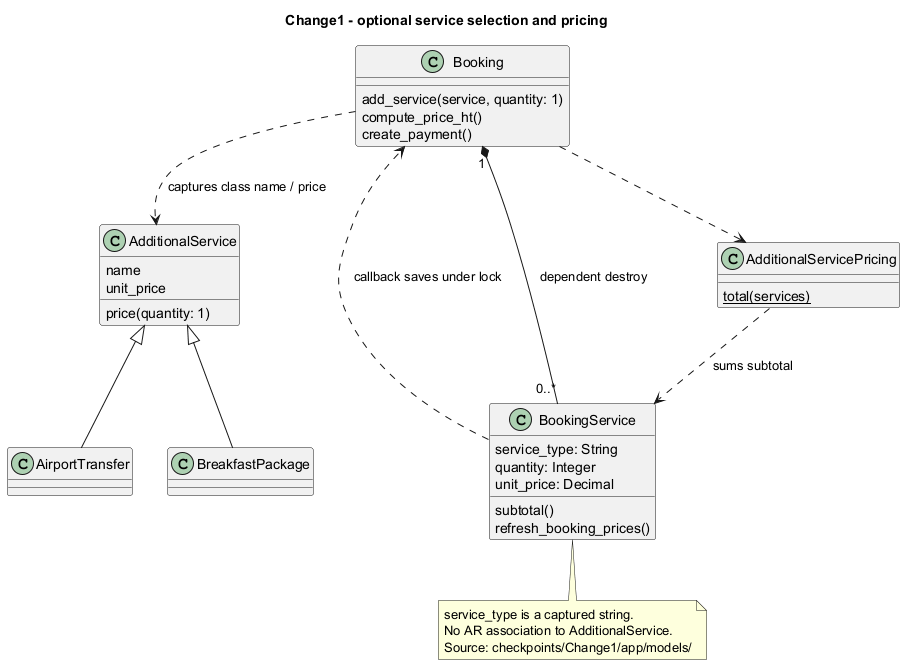
\includegraphics[width=0.78\linewidth]{Part2/diagrams/additional_services.png}
\caption{Additional-service design for breakfast and airport transfer.}
\label{fig:additional-services}
\end{figure}

The key design decision is domain modeling, not pattern labeling. The abstraction allows optional services to grow without turning the core booking record into a list of unrelated boolean or numeric attributes.

The implementation also separates pricing calculation from the controller workflow. The booking total can be expressed as the base accommodation amount plus the subtotal of selected services. This makes service pricing a domain concern that can be tested independently.

The design is \textbf{not} classified as Decorator, Composite, Strategy or Factory. Although the service abstraction could be combined with other patterns in a larger system, the implemented structure does not require those pattern claims.

\paragraph{CH01 acceptance and before/after record.}
Observable criteria are captured service type/price/quantity, persisted selection with a booking foreign key, independent subtotals, refresh after quantity changes/removal, unchanged captured prices, refreshed pending-payment amount/identity and unchanged paid-payment amount. The complete criteria are \code{Part2/changes/Change1/requirement.md}. Before: \code{Part2/checkpoints/original/}; after: \code{Part2/checkpoints/Change1/}; exact changed paths/content: \code{Part2/changes/Change1/diff.patch}. New records/pricing and changes to Booking/HasPriceConcern address responsibility growth. The original callback's date-change-only guard would miss service-only updates; central recomputation on save corrects that concrete coupling. Template Method's Shared CRUD Controller Workflow remains preserved; no new GoF instance is counted.

Run \code{bundle exec rspec spec --format documentation} from the after-checkpoint. \code{Part2/verification/Change1\_rails.txt} records 13 examples, zero failures, including the same five baseline model and seven feature examples. The before receipt \code{Part2/verification/original\_rails.txt} records 5/0. Under the same application-Ruby scope and Ripper tool, SLOC changes 495 to 556. New feature tests are not retroactively claimed to have run on original code. Shared bundle/eager-loading corrections are explicitly assigned to CH01 and visible in its patch.

\subsection{Change 2 -- Room upgrade}

A room upgrade differs from an additional service because it changes the core reservation target. The operation must:

\begin{enumerate}[leftmargin=*]
\item identify the requested target room;
\item verify that the target room is available for the booking interval;
\item calculate the nightly price difference;
\item change the booking's room;
\item recalculate the booking totals;
\item persist the updated booking; and
\item retain a link to the first original room through \code{upgraded\_from\_room}.
\end{enumerate}

The implementation isolates this workflow in \code{RoomUpgrade}. The service receives a booking and target room, validates the requested change, computes the difference, applies the new room and persists it. Saving the booking runs the pricing callbacks that recalculate totals, including selected service charges. The retained original-room association survives repeated upgrades; it is a reference to the first room, not a complete event-history ledger.

\textbf{Dependency boundary:} Change2 introduces \code{Booking.active} before \code{RoomUpgrade} calls it. The baseline already supports a cancellation timestamp. Change2 also uses the scope in booking availability validation and \code{Room\#booked\_dates}, and rejects upgrades of canceled bookings. Change3 inherits these availability semantics and introduces the refund Strategy. The complete Change2 checkpoint is therefore runnable without Change3 classes or its refund migration.

This avoids adding a large conditional branch to \code{Booking\#cancel!} or to controller actions. It also keeps the semantic distinction between ``an optional service attached to a booking'' and ``a replacement of the room being booked.''

The operation is not classified as Command, State or Strategy. The presence of an operation object does not automatically create Command; the implementation is primarily a domain responsibility extraction.

\paragraph{CH02 acceptance and before/after record.}
The target rejects overlapping active stays without changing persisted room/totals, allows adjacent or canceled stays, computes the nightly pre-VAT difference, recalculates total/payment amounts, retains services and the first original room, rolls back invalid changes and rejects canceled-booking upgrades. Complete criteria: \code{Part2/changes/Change2/requirement.md}. Before: \code{Part2/checkpoints/Change1/}; after: \code{Part2/checkpoints/Change2/}; exact source delta: \code{Part2/changes/Change2/diff.patch}. The operation/scope extract new workflow responsibilities from an already broad Booking model. Availability queries still occur in both Booking validation and RoomUpgrade; duplication remains, rather than being claimed eliminated. Template Method is preserved; no new GoF instance is counted.

Run the same complete RSpec command from Change2. \code{Part2/verification/Change2\_rails.txt} records 21/0, including all earlier examples and eight upgrade examples; the before-stage receipt records 13/0. Same-scope SLOC changes 556 to 596. Confirmed reservation means persisted, not necessarily paid. RoomUpgrade is a callable domain service; no upgrade controller route or external upgrade payment is claimed.

\begin{figure}[H]
\centering
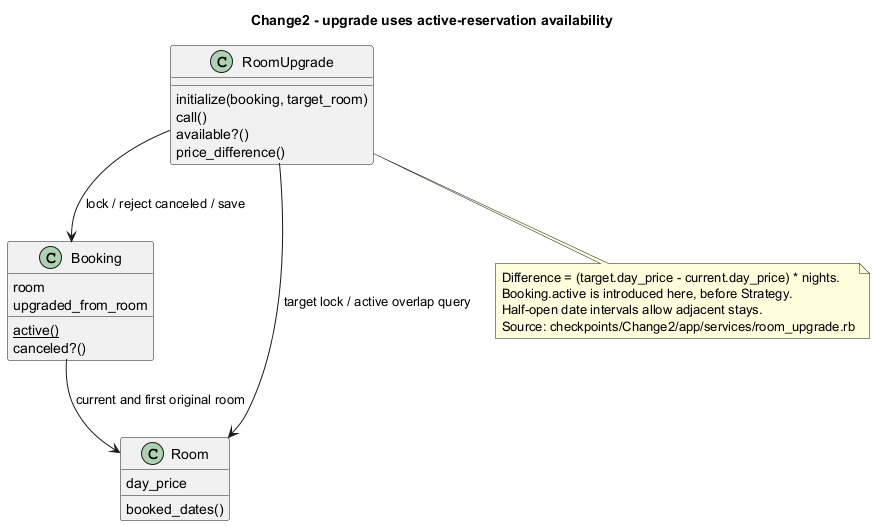
\includegraphics[width=0.85\linewidth,height=0.42\textheight,keepaspectratio]{Part2/diagrams/room_upgrade.png}
\caption{Change2 room upgrade and its active-reservation dependency. Editable source: Part2/diagrams/room\_upgrade.puml.}
\end{figure}

\subsection{Change 3 -- Cancellation Strategy}

Cancellation is different because the business rule can vary while the overall cancellation workflow remains stable. A hotel may offer flexible cancellation, partial refund, or no refund. The core application should not need a growing conditional tree such as:

\begin{lstlisting}[caption={Illustrative anti-pattern avoided by the evolution}]
if policy == "flexible"
  ...
elsif policy == "partial"
  ...
elsif policy == "none"
  ...
end
\end{lstlisting}

Instead, the evolved design uses:

\begin{figure}[H]
\centering
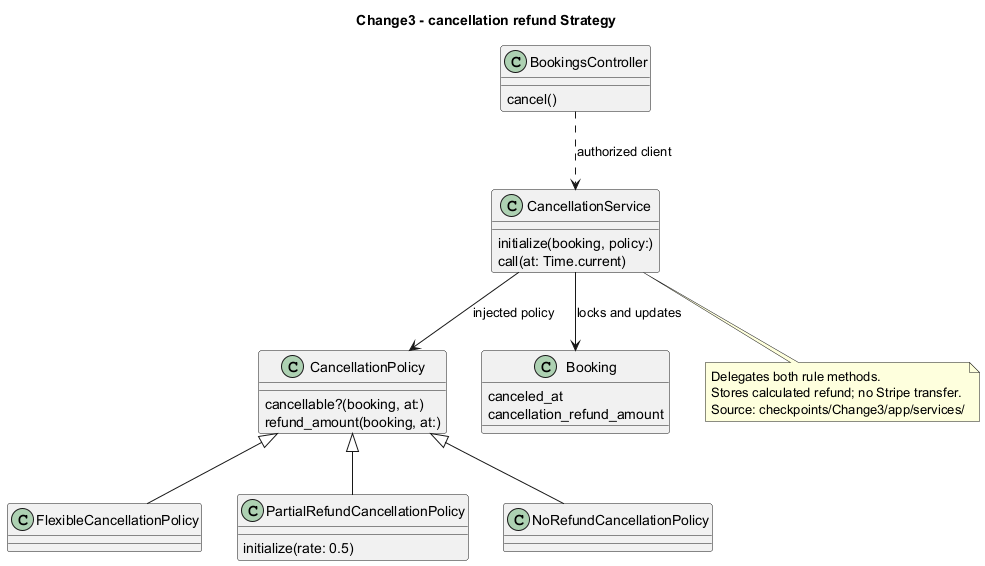
\includegraphics[width=0.72\linewidth]{Part2/diagrams/cancellation_strategy.png}
\caption{Cancellation Strategy collaboration.}
\label{fig:cancellation-strategy}
\end{figure}

The context is \code{CancellationService}. The Strategy interface is \code{CancellationPolicy}. The concrete strategies are:

\begin{itemize}[leftmargin=*]
\item \code{FlexibleCancellationPolicy}
\item \code{PartialRefundCancellationPolicy}
\item \code{NoRefundCancellationPolicy}
\end{itemize}

The context delegates two conceptually related business decisions: whether cancellation is permitted and how the refund is calculated. The policy object therefore encapsulates the variable algorithm. The real \code{BookingsController\#cancel} action authenticates the user, retrieves the scoped booking, authorizes it, and obtains a policy from server configuration. The client cannot select a more generous policy through request parameters. \code{CancellationService\#call} locks the booking, rejects repeated cancellation, delegates the rules, and atomically persists \code{canceled\_at} with \code{cancellation\_refund\_amount}. This records a calculated refund; it does not issue a Stripe refund request or alter the paid payment record.

\lstinputlisting[language=Ruby,caption={Evolved Strategy context and delegation from the final source}]{Part2/code/app/services/cancellation_service.rb}

\paragraph{CH03 acceptance and before/after record.}
Configured policies return full, fractional or zero refunds; the context delegates both rule methods, rejects denied/repeated cancellations and atomically records refund/time. The real route authenticates, scopes, authorizes and ignores client policy choices. Services belong to the refund basis; canceled stays inherit CH02 availability semantics. Complete criteria: \code{Part2/changes/Change3/requirement.md}. Before: \code{Part2/checkpoints/Change2/}; after: \code{Part2/checkpoints/Change3/}, identical to final \code{Part2/code/}; exact source delta: \code{Part2/changes/Change3/diff.patch}.

Original cancellation only recorded a timestamp. Refund variation is new: the actual technique introduces Strategy and injects a policy into a separate context, rather than deleting a historical refund conditional that never existed. Cancellation Refund Policy is newly introduced; Shared CRUD Controller Workflow is preserved. Run the same complete RSpec command from Change3. \code{Part2/verification/Change3\_rails.txt} records 36/0, including earlier examples plus nine service and six route examples; before-stage receipt: 21/0. Same-scope SLOC changes 596 to 654. Atomic local recording and unchanged paid-payment records are tested; no external Stripe refund is implemented.

\subsection{Why cancellation is genuinely Strategy}

The classification follows the GoF intent rather than the class names:

\begin{enumerate}[leftmargin=*]
\item There is a family of related algorithms: cancellation/refund rules.
\item The algorithms perform the same conceptual operation for a common context.
\item The context can receive different policy implementations.
\item The context delegates the variable behavior instead of containing all policy branches.
\item A new policy can be added without changing the central cancellation orchestration.
\end{enumerate}

The Strategy collaboration is therefore substantially stronger than the rejected baseline Pundit-as-Strategy candidate.

\begin{figure}[H]
\centering
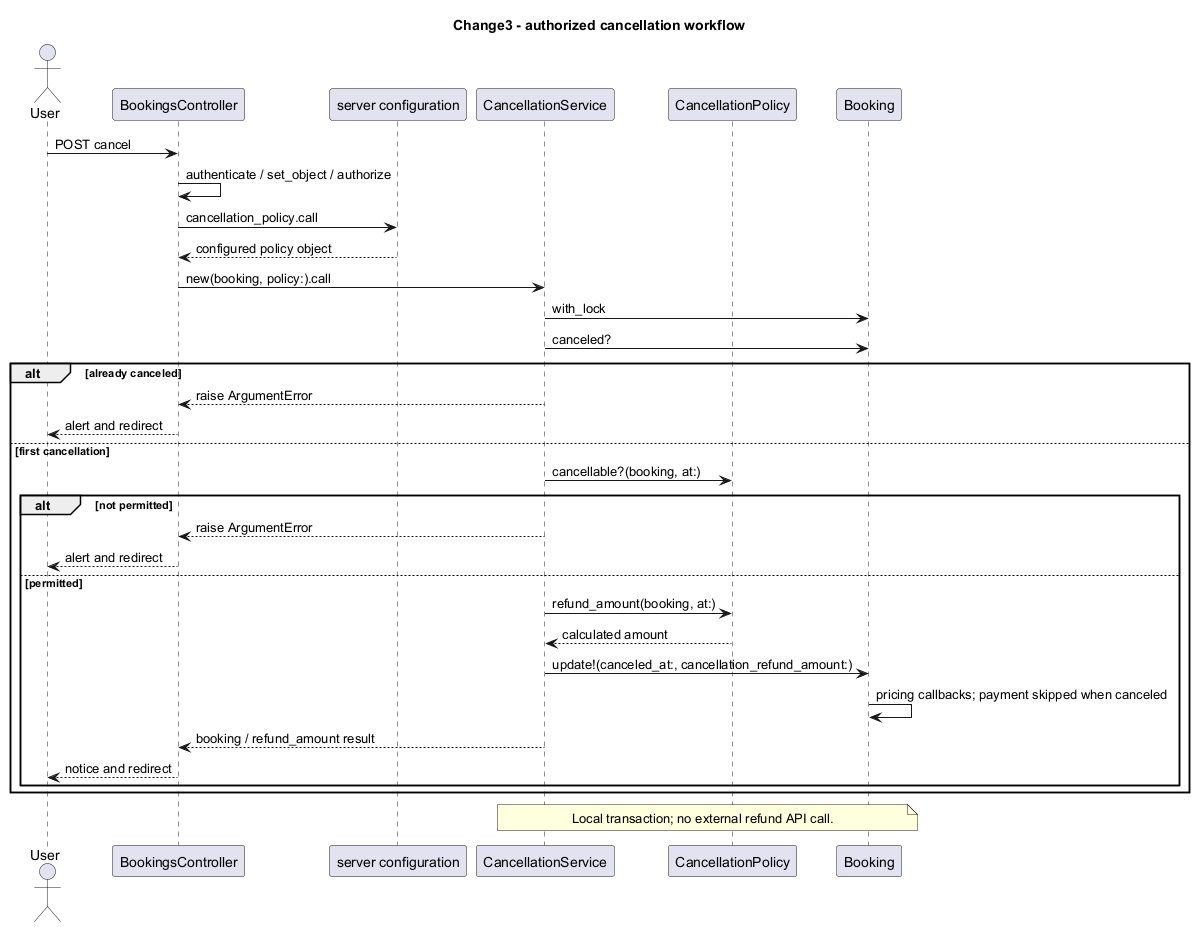
\includegraphics[width=0.83\linewidth]{Part2/diagrams/cancellation_sequence.png}
\caption{Cancellation sequence showing context-to-policy delegation.}
\label{fig:cancellation-sequence}
\end{figure}

\subsection{Before and after architecture}

\begin{figure}[H]
\centering
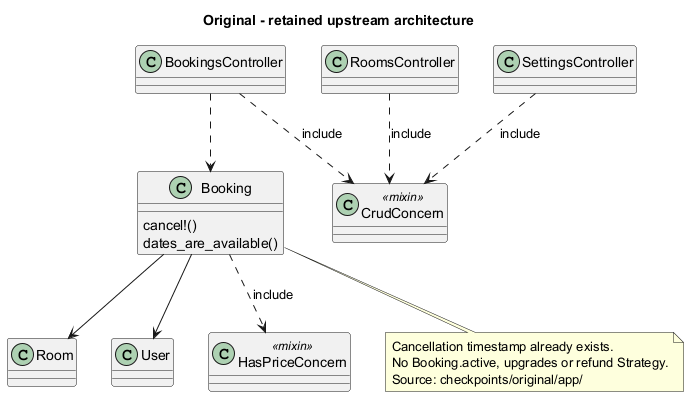
\includegraphics[width=0.85\linewidth,height=0.42\textheight,keepaspectratio]{Part2/diagrams/original_architecture.png}
\caption{Retained original architecture before the three cumulative changes. Editable source: Part2/diagrams/original\_architecture.puml.}
\end{figure}

\begin{figure}[H]
\centering
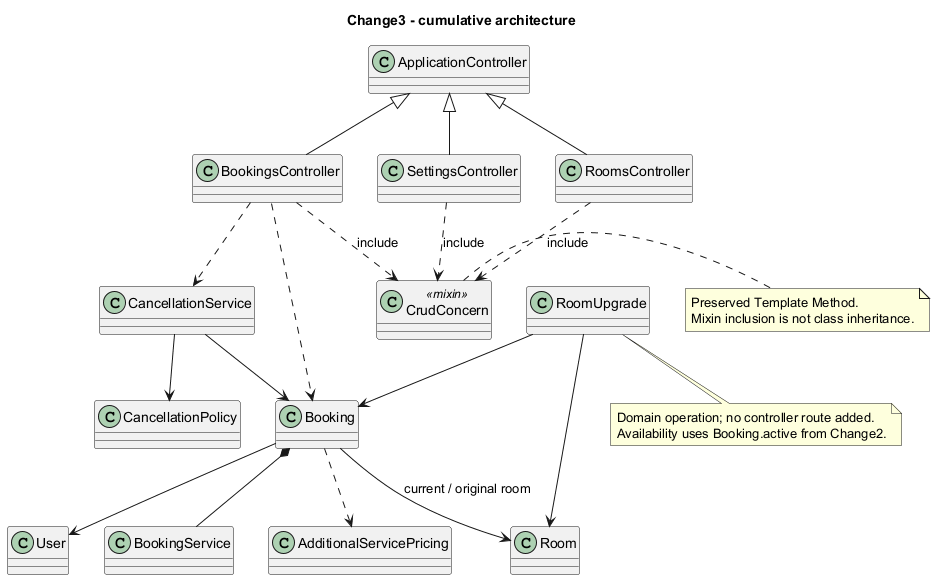
\includegraphics[width=0.84\linewidth]{Part2/diagrams/evolved_architecture.png}
\caption{Evolved architecture with additional services, room upgrade and cancellation policy.}
\label{fig:evolved-architecture}
\end{figure}

The baseline architecture centered most reservation behavior around \code{Booking} and reusable Rails concerns. The evolved architecture introduces explicit application-service/domain boundaries for the new requirements. This is a responsibility-separation decision rather than a claim that every new class is a design pattern.

\subsection{Pattern evolution}

\begin{table}[H]
\centering
\caption{Pattern evolution across the three changes}
\label{tab:evolution}
\begin{tabularx}{\linewidth}{l l X l}
\toprule
Version & Pattern & Instance & Status\\
\midrule
Original & Template Method & Shared CRUD Controller Workflow & Baseline confirmed\\
After Change 1 & Template Method & Shared CRUD Controller Workflow & Preserved\\
After Change 2 & Template Method & Shared CRUD Controller Workflow & Preserved\\
After Change 3 & Template Method & Shared CRUD Controller Workflow & Preserved\\
After Change 3 & Strategy & Cancellation Refund Policy & Newly introduced\\
\bottomrule
\end{tabularx}
\end{table}

The package's evolution CSV records Template Method as preserved and Strategy as newly introduced. \code{Part2/code/} contains the full application with the new models, migrations, application services, server-configured policy selection and real cancellation-route integration. The existing CRUD concern and its resource-specific hooks remain present.

\subsection{Updated participant and observation counts}

\begin{table}[H]
\centering
\caption{Current source-review counts for each saved version}
\begin{tabular}{lrrrrrr}
\toprule
Snapshot & Types & Instances & Concrete classes & Symbols & Rejected & Uncertain\\
\midrule
Original & 1 & 1 & 3 & 4 & 13 & 2\\
Change1 & 1 & 1 & 3 & 4 & 17 & 2\\
Change2 & 1 & 1 & 3 & 4 & 20 & 2\\
Change3 & 2 & 2 & 6 & 10 & 21 & 2\\
\bottomrule
\end{tabular}
\end{table}

Counts come from \code{Part2/evidence/snapshot\_summary.csv} and \code{Part2/evidence/pattern\_observations.csv}, reproduced by \code{tools/summarize\_part2.py}. Three controllers implement Template Method's variable roles; Change3 adds three concrete refund policies. Original has four unique mapped symbols (concern plus controllers); final has ten (those four, five Strategy classes, configured policy callable). Shared BookingsController counts once. This counts named participants, not every method call or application class.

Rejected/uncertain totals are current documented candidate observations within each source scope, not distinct pattern types or recovered historical review events. Dependency Adapter/Facade claims remain uncertain because internals were excluded; other recorded candidates are rejected in the application scope. Optional-service and upgrade guesses remain rejected even when a separate cancellation collaboration becomes confirmed Strategy. Each observation has reasons and bounded source references; no minimum pattern quota is imposed.

\subsection{Refactoring analysis}

The primary design pressure is responsibility growth. The original Booking model already combines associations, availability validation, cancellation state, pricing behavior via a concern, payment integration and notification behavior. New requirements would increase this concentration if implemented directly in the model and controllers.

The evolution responds by extracting responsibilities:

\begin{itemize}[leftmargin=*]
\item additional-service selection and pricing become explicit domain concepts;
\item room-upgrade validation and price adjustment become a dedicated operation;
\item cancellation rules become interchangeable policies;
\item the existing controller Template Method remains responsible for the common CRUD lifecycle.
\end{itemize}

The resulting design is not claimed to be universally superior. It introduces more classes and indirection. That trade-off is justified only when the business rules are expected to vary or grow.

\subsection{Measured before/after source metrics}

\code{tools/measure\_part2.py} invokes Ruby Ripper through \code{tools/ruby\_metrics.rb} on every application Ruby file in each checkpoint. \code{Part2/metrics/before\_after.csv} records per-file source paths and SHA-256 values; \code{Part2/metrics/ruby\_ast\_metrics.json} records method names, source lines, decisions and explicit application dependencies.

\begin{table}[H]
\centering
\caption{Measured cumulative application source (app Ruby files only)}
\begin{tabular}{lrrrrr}
\toprule
Stage & SLOC & Methods & Sum method CC & Max CC & Explicit refs.\\
\midrule
Original & 495 & 95 & 127 & 4 & 27\\
Change1 & 556 & 105 & 145 & 5 & 31\\
Change2 & 596 & 110 & 154 & 6 & 31\\
Change3 & 654 & 121 & 171 & 6 & 35\\
\bottomrule
\end{tabular}
\end{table}

SLOC excludes blank and comment-only lines. Method CC starts at one and counts AST conditionals (including elsif), loops, ternaries, each case/rescue branch and short-circuit Boolean decisions; blocks belong to their enclosing method. Explicit references are a bounded coupling proxy: distinct application-owned constant references per file, summed across files. They exclude declarations and do not capture implicit Rails associations, framework or runtime-dispatch dependencies. The complete rules are in \code{Part2/metrics/README.md}.

These measurements describe cumulative requirements, not equivalent competing implementations. Source size, total method complexity and explicit references increase. Responsibility separation and Strategy do not establish an overall numerical complexity reduction or runtime performance improvement. All Part2 diagrams now have editable PlantUML sources alongside their rendered images, including original architecture and Change2 room upgrade.

\subsection{Part 2 verification status}

Fresh repair verification used Ruby 2.7.5 and the checkpoint bundles with an isolated PostgreSQL server. Separate checkpoint databases were created and migrated; the final full RSpec suite passed \textbf{36 examples, zero failures}. This total comprises five baseline model examples, 30 feature examples and one eager-loading example. Cumulative checkpoint suites report original: 5/0, Change1: 13/0, Change2: 21/0 and Change3: 36/0. Change3 includes nine cancellation service examples and six real cancellation-route request examples. Actual command/output/exit-code receipts are in \code{Part2/verification/}; \code{tools/run\_part2\_tests.ps1} reproduces them. Earlier retained feature receipts (7/0, 8/0, 15/0) and HTTP/boot logs remain historical artifacts and are not presented as fresh runs or as historical executions of the reconstructed stages.

\begin{table}[H]
\centering
\caption{Fresh suite receipt and retained earlier Rails verification artifacts}
\begin{tabularx}{\linewidth}{lX}
\toprule
Verification & Retained evidence\\
\midrule
Fresh final suite: 36/0 & \code{Part2/verification/final\_rails.txt}\\
Complete RSpec suite: 36/0 & \code{test\_result/part2\_rspec.txt}\\
Clean migration rebuild & \code{test\_result/test\_db\_migrations.txt}\\
Twelve migrations up & \code{test\_result/test\_db\_migration\_status.txt}\\
Independent Rails runner boot & \code{test\_result/rails\_boot.txt}: Rails 7.0.6, test environment, 11 tables, exit zero\\
Real Puma HTTP startup & \code{test\_result/rails\_http\_boot.txt}: GET / returns HTTP 302 with location /fr\\
Feature tests by change & \code{Part2/changes/Change1/test\_result.txt}\newline \code{Part2/changes/Change2/test\_result.txt}\newline \code{Part2/changes/Change3/test\_result.txt}\\
Regression before fixes: 30/27 & \code{test\_result/part2\_regression\_before.txt}\\
Boot regression before fix: 1/1 & \code{test\_result/boot\_regression\_before.txt}\\
\bottomrule
\end{tabularx}
\end{table}

The suite exercises persisted room upgrades, original-room retention, availability boundaries, service totals, cancellation state/refund recording, configured policy selection, authentication, ownership and repeated cancellation. The eager-loading check required explicitly declaring \code{active\_model\_serializers}, a dependency used by the upstream Payify integration; this support is assigned to reconstructed Change1. The logs contain duplicate-constant warnings from \code{net/protocol}; fresh successful test and migration commands exit zero. Earlier HTTP/boot logs in the table are retained artifacts, not rerun proof. Production deployment and external payment/webhook delivery remain outside the verification scope.

% ---------------- PART 3 ----------------
\section{Part 3 -- Cross-language Comparison}

\subsection{Purpose and scope}

The cross-language exercise does not attempt to port the complete Rails application. It isolates the two confirmed design ideas and reproduces their representative behavior:

\begin{itemize}[leftmargin=*]
\item Template Method: a shared resource-rendering/CRUD-style workflow with resource-specific hooks.
\item Strategy: cancellation refund behavior selected through a policy object.
\end{itemize}

The purpose is to compare how different languages express abstraction, inheritance, interfaces, dynamic dispatch and ownership while preserving the same design intent.

\subsection{Shared behavioral specifications}

For Template Method, the common workflow creates a resource-specific representation using hooks for Booking, Room and Settings. The common algorithm remains in the template while the concrete resource implementations supply details.

For Strategy, a booking amount of 430 is passed to three policies. The expected outputs are:

\begin{table}[H]
\centering
\caption{Strategy behavioral specification}
\label{tab:strategy-spec}
\begin{tabular}{lll}
\toprule
Policy & Rule & Expected refund\\
\midrule
Flexible & Full eligible refund & 430\\
Partial refund & 50\% refund & 215\\
No refund & No refund & 0\\
\bottomrule
\end{tabular}
\end{table}

All four language implementations use the same representative behavior.

\subsection{Template Method mapping}

\begin{table}[H]
\centering
\caption{Template Method mapping across languages}
\label{tab:tm-language}
\begin{tabularx}{\linewidth}{lXX}
\toprule
Language & Main abstraction & Language-specific expression\\
\midrule
Ruby & \code{CrudConcern} & ActiveSupport concern with shared workflow and hook methods.\\
Java & Abstract/template workflow class & Explicit abstract methods/interfaces and static typing.\\
Python & ABC-based workflow & Abstract base class and dynamic dispatch.\\
JavaScript & Base workflow class & Runtime polymorphism through class methods.\\
C++ & Abstract base class & Pure virtual functions and virtual dispatch.\\
\bottomrule
\end{tabularx}
\end{table}

The language implementations are analogous, not source-identical. Ruby's concern mechanism is especially different from the other four because the original application integrates shared behavior through a module included into controllers.

\subsection{Strategy mapping}

\begin{table}[H]
\centering
\caption{Strategy mapping across languages}
\label{tab:strategy-language}
\begin{tabularx}{\linewidth}{lXX}
\toprule
Language & Strategy abstraction & Concrete policies\\
\midrule
Java & Policy interface/abstract contract & Flexible, PartialRefund, NoRefund\\
Python & ABC-based policy contract & Flexible, PartialRefund, NoRefund\\
JavaScript & Base policy class & Flexible, PartialRefund, NoRefund\\
C++ & Abstract policy class / shared ownership & Flexible, PartialRefund, NoRefund\\
\bottomrule
\end{tabularx}
\end{table}

The common structure is:

\begin{center}
\code{CancellationService -> CancellationPolicy -> Flexible / PartialRefund / NoRefund}
\end{center}

The important cross-language invariant is delegation: the service does not encode each refund algorithm directly.

\subsection{Execution results}

Eight snippets were executed: Template Method and Strategy in each of four languages.

\begin{table}[H]
\centering
\caption{Part 3 execution verification}
\label{tab:execution}
\begin{tabular}{llll}
\toprule
Pattern & Language & Command family & Result\\
\midrule
Template Method & Java & \code{javac Main.java \&\& java Main} & Passed 1/1\\
Template Method & Python & \code{python3 Main.py} & Passed 1/1\\
Template Method & JavaScript & \code{node Main.js} & Passed 1/1\\
Template Method & C++ & \code{g++ -std=c++17 ... \&\& ./main} & Passed 1/1\\
Strategy & Java & \code{javac Main.java \&\& java Main} & Passed 1/1\\
Strategy & Python & \code{python3 Main.py} & Passed 1/1\\
Strategy & JavaScript & \code{node Main.js} & Passed 1/1\\
Strategy & C++ & \code{g++ -std=c++17 ... \&\& ./main} & Passed 1/1\\
\bottomrule
\end{tabular}
\end{table}

The test results are behavioral smoke checks for the isolated snippets, not proof that the complete Rails application behaves identically across languages.

\subsection{Static comparison}

The official cross-language dataset reports the following source LOC and maximum function cyclomatic complexity:

\begin{table}[H]
\centering
\caption{Cross-language static metrics}
\label{tab:static}
\begin{tabular}{llrr}
\toprule
Pattern & Language & Source LOC & Max function CC\\
\midrule
Template Method & Java & 9 & 1\\
Template Method & Python & 17 & 1\\
Template Method & JavaScript & 9 & 1\\
Template Method & C++ & 9 & 2\\
Strategy & Java & 6 & 1\\
Strategy & Python & 14 & 1\\
Strategy & JavaScript & 6 & 1\\
Strategy & C++ & 9 & 2\\
\bottomrule
\end{tabular}
\end{table}

LOC excludes blank lines and comments according to the project measurement convention. The low cyclomatic complexity reflects that the examples intentionally isolate pattern structure rather than application-scale business logic.

\subsection{Performance measurements}

Each snippet was measured using one warmup process followed by five measured process runs. The median process time is reported. Timing includes process startup and snippet execution.

\begin{table}[H]
\centering
\caption{Median process-level timing}
\label{tab:timing}
\begin{tabular}{lrr}
\toprule
Language & Template Method (ms) & Strategy (ms)\\
\midrule
Java & 39.494 & 50.372\\
Python & 672.008 & 595.258\\
JavaScript & 21.401 & 21.762\\
C++ & 1.097 & 1.223\\
\bottomrule
\end{tabular}
\end{table}

These measurements should not be interpreted as a universal language benchmark. The examples are tiny, and process startup can dominate their runtime. The useful conclusion is narrower: the same structural pattern can be implemented and executed in all four languages, while language/runtime characteristics produce different observed process-level timings.

\subsection{Language-specific observations}

\paragraph{Java.}
Java makes the pattern contracts explicit through interfaces and abstract classes. Static typing makes participant relationships visible in declarations, at the cost of more syntactic structure.

\paragraph{Python.}
Python can express the same abstraction using ABCs, but its dynamic dispatch makes some contracts less syntactically prominent. The implementation is concise in conceptual terms while retaining explicit abstract methods.

\paragraph{JavaScript.}
JavaScript's class syntax provides a familiar object-oriented surface, but dispatch remains dynamic. The pattern can be expressed without compile-time interface enforcement.

\paragraph{C++.}
C++ expresses the abstraction through pure virtual functions and runtime virtual dispatch. The implementation can also use ownership mechanisms such as \code{shared\_ptr} for the selected Strategy.

% ---------------- LLM ----------------
\section{LLM Records and Human Verification}

\subsection{Role of LLM assistance}

LLMs were used as analytical assistants in several project stages:

\begin{enumerate}[leftmargin=*]
\item baseline source analysis;
\item architecture extraction;
\item pattern discovery;
\item evolution analysis;
\item cross-language implementation;
\item final audit.
\end{enumerate}

The methodological boundary was that an LLM output was treated as a hypothesis rather than as primary evidence.



\subsection{Retained records}

The package retains six analysis stages. Prompt 01 and Prompts 04--06 are preserved as prompt records. The exact historical wording for Prompts 02 and 03 could not be recovered as independent verbatim records. Rather than reconstructing those prompts and presenting the reconstruction as historical evidence, the package records the limitation.

Historical model/date metadata is also marked unknown where it could not be independently verified.

\begin{table}[H]
\centering
\caption{LLM evidence and verification status}
\label{tab:llm}
\begin{tabularx}{\linewidth}{lXX}
\toprule
Stage & Retained evidence & Verification\\
\midrule
Pattern discovery & Source-analysis result and evidence matrix & Source locations checked independently.\\
Evolution & Evolution analysis, change diffs and Rails receipts & Full Rails suite: 36 examples, zero failures.\\
Cross-language & Four-language implementations and result analysis & Eight snippets independently executed.\\
Final audit & Audit result and submission checklist & Package structure and evidence cross-checked.\\
Prompt 02/03 history & Verbatim historical records unavailable & Explicitly not reconstructed.\\
\bottomrule
\end{tabularx}
\end{table}

\subsection{Human verification}

Verification consisted of source inspection, participant mapping, candidate rejection, code execution where possible, and numerical cross-checking.

The most important human-verification outcomes were:

\begin{itemize}[leftmargin=*]
\item Template Method was confirmed from concrete source interactions.
\item Pundit was not inflated into Strategy.
\item callbacks were not inflated into Observer.
\item Payify was not inflated into Adapter/Facade.
\item concerns were not inflated into Decorator.
\item Part 2 Strategy was implemented as actual delegation rather than inferred from a class name.
\item Part 3 timing values were collected rather than invented.
\end{itemize}

% ---------------- LIMITATIONS ----------------
\section{Limitations}

A defensible case study must state the boundaries of its evidence.

\begin{enumerate}[leftmargin=*]
\item \textbf{External payment internals.} Payify/Stripe internals are not fully observable from the application source, so their internal design patterns are not classified.
\item \textbf{External webhook internals.} Integromat/Make behavior outside the application's webhook invocation is not observable.
\item \textbf{Representative Part 3 scope.} The four-language examples are representative pattern implementations, not full Rails ports.
\item \textbf{Simplified business behavior.} Cross-language examples simplify application-scale concerns such as persistence, date availability, money representation and cancellation timing.
\item \textbf{Test environment scope.} Migrations, persisted feature behavior, model tests, actual-route requests and eager loading were verified on a dedicated PostgreSQL test database. Production deployment and live external-service operation were not exercised.
\item \textbf{Refund delivery scope.} Cancellation persists the calculated refund amount and timestamp. It does not issue an external Stripe refund or claim settlement of money.
\item \textbf{Timing scope.} Process-level timings include startup and are based on tiny programs. They are comparative observations, not language benchmarks.
\item \textbf{Historical LLM metadata.} Some historical model/date information is unavailable and therefore remains explicitly unknown.
\item \textbf{Historical Prompt 02/03 wording.} Exact verbatim records were not retained and were not reconstructed.
\item \textbf{Team contribution evidence.} Kurt Sony Rebello's primary contribution is documented in the project brief. The retained records do not independently document specific technical contributions for the other three students; the report therefore does not fabricate task assignments for them.
\end{enumerate}

% ---------------- FINDINGS ----------------
\section{Findings and Contributions}

\subsection{Finding 1 -- A single baseline pattern is defensible}

The original application contains one clearly evidenced application-level GoF collaboration: Template Method through \code{CrudConcern} and its concrete controllers. This conclusion is narrower than a pattern-by-name inventory but stronger because the participant roles and calls can be traced directly.

\subsection{Finding 2 -- False positives matter}

Several Rails mechanisms resemble classic patterns. However, similarity of vocabulary is insufficient. Pundit policies are authorization constructs; callbacks are lifecycle hooks; concerns are a Ruby/Rails reuse mechanism; and Payify is an external payment dependency. None was promoted to a GoF pattern without the required collaboration evidence.

\subsection{Finding 3 -- Requirements create different design pressures}

Breakfast and airport transfer are best understood as optional service domain concepts. Room upgrade is a reservation modification workflow. Cancellation policy is a variable business-rule family. Treating these requirements identically would obscure their different design pressures.

\subsection{Finding 4 -- Cancellation is a strong Strategy case}

The cancellation requirement creates interchangeable algorithms with a stable context. \code{CancellationService} delegates to \code{CancellationPolicy}, allowing flexible, partial-refund and no-refund implementations. This is the strongest new pattern introduced by the evolution.

\subsection{Finding 5 -- Cross-language mechanisms differ}

The same design intent appears through Java interfaces/abstract classes, Python ABCs, JavaScript class-based dynamic dispatch and C++ pure virtual functions. The pattern concept is therefore more stable than its language-level expression.

\subsection{Finding 6 -- Evidence reduces pattern inflation}

The project demonstrates a general methodological lesson: a defensible design-pattern inventory should be willing to contain only one baseline pattern when only one collaboration is actually established. Academic quality is improved by rejecting unsupported candidates rather than maximizing the pattern count.

\subsection{Contributions}

The inherited report attributed the overall case-study work primarily to Kurt Sony Rebello. The supporting project brief and independent contribution evidence are unavailable in the supplied inputs, so this repair cannot confirm that historical attribution. It is not presented as a verified contribution record.

For Kavya Penikalapati, E. Abhijith Krishna and Guduru Akshaya Giri, the retained project records available for this report do not contain independently verified, specific technical contribution assignments. Their names and team membership are therefore reported exactly, but no unsupported technical tasks are attributed to them.

% ---------------- CONCLUSION ----------------
\section{Conclusion}

This case study examined an existing Ruby on Rails hotel booking application using a source-first, evidence-based design-pattern methodology. The baseline was fixed to an immutable commit so that the pattern inventory could be reproduced against a defined source state. The architecture was analyzed as a Rails MVC/Active Record system with controllers, models, concerns and external integrations.

The baseline result was intentionally conservative: one application-level GoF collaboration, Template Method, was confirmed. \code{CrudConcern} provides a common CRUD algorithm and concrete resource controllers supply resource-specific hooks. The source locations, interactions and behavioral purpose support the classification. Several other plausible candidates were investigated but rejected because the required pattern collaboration was not established.

The evolution phase demonstrated that new requirements do not imply a uniform pattern solution. Breakfast and airport transfer were modeled as additional services. Room upgrade was isolated as a domain operation. Cancellation policy introduced genuine algorithmic variation and was therefore represented using Strategy. \code{CancellationService} acts as the context and delegates cancellation/refund behavior to interchangeable policy implementations.

The cross-language phase showed that the same design intent can be represented in Java, Python, JavaScript and C++. All eight representative snippets passed their behavioral checks. Process-level timing measurements were collected using one warmup and five measured runs, and the medians were reported. The measurements demonstrate environmental/runtime differences but do not establish universal language performance rankings.

The most important lesson is methodological. Design patterns should be identified from collaborations and intent, not from names or superficial structural resemblance. Likewise, evolution should introduce a pattern only when the new requirement creates the problem that the pattern is designed to solve. The resulting architecture is not claimed to be universally superior: it trades some additional classes and indirection for clearer separation of variable business rules.

Overall, the case study shows how a real Rails application can be analyzed, challenged, evolved and reproduced across languages while maintaining a clear distinction between framework mechanisms, domain design and recognized GoF patterns.

% ---------------- REFERENCES ----------------
\section{References}

\begin{enumerate}[leftmargin=*]
\item Andrew D. Silva, \emph{rails-room-booking}, GitHub repository, baseline commit \baseline. \repo
\item E. Gamma, R. Helm, R. Johnson and J. Vlissides, \emph{Design Patterns: Elements of Reusable Object-Oriented Software}, Addison-Wesley, 1994.
\item Ruby on Rails, \emph{Rails Guides: Getting Started, Active Record and Active Support}, official Rails documentation.
\item Pundit, \emph{Pundit Authorization for Ruby Applications}, project documentation.
\item Devise, \emph{Flexible authentication solution for Rails}, project documentation.
\item Payify, payment integration dependency referenced by the baseline application.
\item Stripe, \emph{Stripe API Documentation}, payment platform documentation.
\item PlantUML, \emph{PlantUML Language Reference Guide}, documentation for editable UML diagrams.
\item Java Platform Documentation, OpenJDK API and language documentation.
\item Python Documentation, Python language and standard-library documentation.
\item Node.js Documentation, JavaScript runtime documentation.
\item ISO/IEC 14882, \emph{Programming Languages -- C++}, C++ language standard family.
\end{enumerate}

% ---------------- APPENDICES ----------------
\appendix
\section{Detailed Source Evidence}

\subsection{CrudConcern evidence}

The verified baseline \code{CrudConcern} contains the common CRUD algorithm and the hook methods used by the concrete controllers. The source is \code{code/app/controllers/concerns/crud\_concern.rb:1--149}. The critical structural evidence is:

\begin{lstlisting}[language=Ruby,caption={Core Template Method structure in CrudConcern}]
def create
  authorize object_class
  @object = object_class.new(form_values)

  if @object.valid?
    @object.save!
    redirect_to_show(@object)
  else
    render :new, status: :unprocessable_entity
  end
end

private

def base_class
  raise NotImplementedError
end

def object_class
  raise NotImplementedError
end
\end{lstlisting}

The same concern supplies \code{index}, \code{show}, \code{new}, \code{edit}, \code{update} and \code{destroy}. The concrete controllers then specialize the hook methods.

\subsection{Booking evidence}

The baseline Booking source establishes:

\begin{itemize}[leftmargin=*]
\item \code{belongs\_to :user}
\item \code{belongs\_to :room}
\item validation of dates, room and user
\item date-conflict validation
\item payment state queries
\item cancellation through \code{canceled\_at}
\item price access through \code{total\_ttc}
\item \code{after\_save :create\_payment}
\item \code{after\_create :notify\_booking}
\end{itemize}

The cancellation implementation is intentionally simple:

\begin{lstlisting}[language=Ruby,caption={Baseline cancellation behavior}]
def cancel!
  update_attribute :canceled_at, Time.now
end
\end{lstlisting}

This is why cancellation policy is treated as a new evolution requirement rather than as an existing baseline Strategy.

\section{Part 2 Change Acceptance}

\subsection{Change 1 acceptance}

The implementation is considered structurally satisfied when a booking can be associated with breakfast or airport-transfer service objects/records and the service subtotal participates in the total calculation without modifying the original room amenity list.

\subsection{Change 2 acceptance}

The room-upgrade operation must reject an unavailable target room, calculate the target/base price difference, replace the booking room when valid, and recalculate the booking total.

\subsection{Change 3 acceptance}

The cancellation context must accept a policy, delegate the eligibility/refund operation to that policy, and support at least flexible, partial-refund and no-refund concrete policies without embedding all algorithms in the context.

\section{Cross-language Test Specification}

The representative Strategy input is a booking amount of 430. Expected output is 430 for flexible cancellation, 215 for a 50\% partial refund, and 0 for no refund. The Template Method example must demonstrate that a common workflow is reused while Booking, Room and Settings supply different resource-specific output.

The execution evidence stored under \code{Part3/evidence/} records the actual output for each language. The official \code{data/cross\_language.csv} records source LOC, maximum function cyclomatic complexity, runtime/compiler, command, result, median process time and language notes.

\section{Submission and Evidence Audit}

\begin{table}[H]
\centering
\caption{Final evidence audit}
\label{tab:audit}
\begin{tabularx}{\linewidth}{lXl}
\toprule
Item & Evidence & Status\\
\midrule
Team metadata & Master project brief & Verified\\
Baseline commit & Original GitHub repository & Verified\\
Baseline pattern count & \code{data/pattern\_counts.csv} + source evidence & Verified\\
Template Method evidence & Source paths and participant mapping & Verified\\
Part 2 changes & Full evolved Rails application, migrations and RSpec receipts & 36 examples, zero failures\\
Strategy implementation & Context, abstract contract and three concrete policies & 9 service + 6 request examples passed\\
Part 3 tests & Eight snippets & Passed 1/1 each\\
Performance measurements & \code{data/cross\_language.csv} + raw evidence & Verified\\
LLM records & \code{data/llm.csv} and retained prompts/results & Partial; historical metadata gaps disclosed\\
Prompt 02/03 verbatim history & Not retained & Not verified\\
\bottomrule
\end{tabularx}
\end{table}

\end{document}
